\section{Paradigm Discussion}
\label{sec:paradigm}



\subsection{The Intelligent Compute Core: From Silicon to Substrate}

The preceding sections established the ICA analogy framework and its layered architecture. Figure~\ref{fig:paradigm_timeline} summarizes the structural parallels between classical CPU evolution and LLM system development. This subsection examines the core itself: the large language model as \textit{processor} within an intelligent system, and how five decades of CPU evolution illuminate its trajectory. The argument proceeds through six stages: what the core is, how it scales, how heterogeneous designs circumvent scaling limits, what specialized units surround it, what substrates might eventually replace silicon, and how to measure whether it works.

\begin{figure}[t]
\centering
\resizebox{\textwidth}{!}{%
\begin{tikzpicture}[
    font=\sffamily,
    >=Stealth,
    % ---- Node styles ----
    cpuNode/.style={
        draw=classical!80, fill=classical!18,
        rounded corners=3pt,
        minimum width=22mm, minimum height=9mm,
        inner sep=2pt, align=center,
        font=\scriptsize\bfseries, text=classical!90!black,
        line width=0.6pt
    },
    llmNode/.style={
        draw=modelnative!80, fill=modelnative!18,
        rounded corners=3pt,
        minimum width=22mm, minimum height=9mm,
        inner sep=2pt, align=center,
        font=\scriptsize\bfseries, text=modelnative!90!black,
        line width=0.6pt
    },
    futureNode/.style={
        draw=modelnative!60, fill=modelnative!8,
        rounded corners=3pt,
        minimum width=22mm, minimum height=9mm,
        inner sep=2pt, align=center,
        font=\scriptsize\bfseries\itshape, text=modelnative!70!black,
        line width=0.6pt, dashed
    },
    yearLabel/.style={
        font=\tiny\bfseries, text=timelineGray!85!black
    },
    timelineLine/.style={
        line width=1.6pt, draw=#1!50
    },
    phaseBand/.style={
        fill=#1, fill opacity=0.08, rounded corners=4pt
    },
    curvedArrow/.style={
        -{Stealth[length=2.2mm, width=1.5mm]},
        thick, draw=#1,
        shorten <=2pt, shorten >=2pt
    },
    arrowLabel/.style={
        font=\tiny\bfseries, text=#1,
        fill=white, fill opacity=0.85, text opacity=1,
        rounded corners=1.5pt, inner xsep=3pt, inner ysep=1.2pt,
        draw=#1!30, line width=0.3pt
    },
    timelineHeader/.style={
        font=\small\bfseries, text=#1,
        fill=#1!6, rounded corners=3pt, inner sep=4pt
    }
]

% ==============================================================
%  COORDINATE SYSTEM
%  x-axis: logical year position (evenly spaced for clarity)
%    CPU:  x = 0, 3, 6, 9, 12, 15, 18
%    LLM:  x = 0, 3, 6, 6, 9, 9, 12   (some share year positions)
%  y-axis:
%    CPU timeline at y = 2.8
%    LLM timeline at y = -1.2
% ==============================================================
\def\cpuY{2.8}
\def\llmY{-1.2}

% ==============================================================
%  PHASE BACKGROUND BANDS
% ==============================================================
% CPU Phase 1: Sequential / Scalar era (1945-2004)
\fill[phaseBand=classical]
    (-1.3, \cpuY+1.1) rectangle (4.7, \cpuY-0.5);
% CPU Phase 2: Parallelism & Heterogeneity (2005-2019)
\fill[phaseBand=classical]
    (4.9, \cpuY+1.1) rectangle (13.7, \cpuY-0.5);
% CPU Phase 3: Specialization (2020+)
\fill[phaseBand=classical]
    (13.9, \cpuY+1.1) rectangle (19.5, \cpuY-0.5);

% LLM Phase 1: Pretrained Foundation (2020)
\fill[phaseBand=modelnative]
    (-1.3, \llmY+0.65) rectangle (1.7, \llmY-1.05);
% LLM Phase 2: Interfaces & Bottlenecks (2023-2024)
\fill[phaseBand=modelnative]
    (1.9, \llmY+0.65) rectangle (7.7, \llmY-1.05);
% LLM Phase 3: Heterogeneous Orchestration (2025-Future)
\fill[phaseBand=modelnative]
    (7.9, \llmY+0.65) rectangle (13.5, \llmY-1.05);

% Phase labels (subtle, inside bands)
\node[font=\tiny\itshape, text=classical!45]
    at (1.7, \cpuY+0.85) {Sequential Era};
\node[font=\tiny\itshape, text=classical!45]
    at (9.3, \cpuY+0.85) {Parallelism \& Heterogeneity};
\node[font=\tiny\itshape, text=classical!45]
    at (16.7, \cpuY+0.85) {Specialization};

\node[font=\tiny\itshape, text=modelnative!45]
    at (0.2, \llmY-0.7) {Foundation};
\node[font=\tiny\itshape, text=modelnative!45]
    at (4.8, \llmY-0.7) {Interfaces \& Bottlenecks};
\node[font=\tiny\itshape, text=modelnative!45]
    at (10.7, \llmY-0.7) {Orchestration \& Specialization};

% ==============================================================
%  TIMELINE HEADERS
% ==============================================================
\node[timelineHeader=classical] at (9, \cpuY+1.55) {CPU Architecture};
\node[timelineHeader=modelnative] at (6, \llmY+1.05) {LLM Systems};

% ==============================================================
%  TIMELINE LINES
% ==============================================================
\draw[timelineLine=classical] (-1.0, \cpuY) -- (19.0, \cpuY);
\draw[timelineLine=modelnative] (-1.0, \llmY) -- (13.0, \llmY);

% ==============================================================
%  CPU TIMELINE MILESTONES  (top row)
% ==============================================================
% 1945: ENIAC
\node[cpuNode] (cpu1) at (0, \cpuY) {ENIAC};
\node[yearLabel, below=2.5mm of cpu1] {1945};

% 1978: x86 ISA
\node[cpuNode] (cpu2) at (3, \cpuY) {x86 ISA};
\node[yearLabel, below=2.5mm of cpu2] {1978};

% 2005: Dennard Scaling Collapse
\node[cpuNode] (cpu3) at (6, \cpuY) {Dennard\\[-1pt]Collapse};
\node[yearLabel, below=2.5mm of cpu3] {2005};

% 2006: Multi-core
\node[cpuNode] (cpu4) at (9, \cpuY) {Multi-core};
\node[yearLabel, below=2.5mm of cpu4] {2006};

% 2012: big.LITTLE
\node[cpuNode] (cpu5) at (12, \cpuY) {big.LITTLE};
\node[yearLabel, below=2.5mm of cpu5] {2012};

% 2016: Heterogeneous SoC
\node[cpuNode] (cpu6) at (15, \cpuY) {Hetero.\\[-1pt]SoC};
\node[yearLabel, below=2.5mm of cpu6] {2016};

% 2020+: Domain-Specific Accelerators
\node[cpuNode] (cpu7) at (18, \cpuY) {Domain\\[-1pt]Accelerators};
\node[yearLabel, below=2.5mm of cpu7] {2020+};

% ==============================================================
%  LLM TIMELINE MILESTONES  (bottom row)
% ==============================================================
% 2020: Pretrained LLMs
\node[llmNode] (llm1) at (0, \llmY) {GPT-3};
\node[yearLabel, above=2.5mm of llm1] {2020};

% 2023: Token/Tool Interface
\node[llmNode] (llm2) at (3, \llmY) {ChatGPT\\[-1pt]Plugins};
\node[yearLabel, above=2.5mm of llm2] {2023};

% 2024: Inference Energy Wall
\node[llmNode] (llm3) at (5.5, \llmY) {KV Cache\\[-1pt]Wall};
\node[yearLabel, above=2.5mm of llm3] {2024};

% 2024: Sparse MoE
\node[llmNode] (llm4) at (8, \llmY) {Sparse\\[-1pt]MoE};
\node[yearLabel, above=2.5mm of llm4] {2024};

% 2025: Heterogeneous Model Orchestration
\node[llmNode] (llm5) at (10.5, \llmY) {Multi-Model\\[-1pt]Orchestr.};
\node[yearLabel, above=2.5mm of llm5] {2025};

% 2025: Specialized Small Models
\node[llmNode] (llm6) at (13, \llmY) {Specialized\\[-1pt]SLMs};
\node[yearLabel, above=2.5mm of llm6] {2025};

% Future: Alternative Substrates  (not connected by arrows; shown for completeness)
% (Omitted to keep the figure focused on the five structural parallels)

% ==============================================================
%  CURVED CONNECTING ARROWS  (CPU → LLM structural parallels)
% ==============================================================
% The arrows curve downward from the CPU timeline to the LLM timeline.
% We use bend left/right to create aesthetically curved paths.

% 1. Dennard Collapse → KV Cache Wall  ("Power Wall")
\draw[curvedArrow=red!70!black]
    (cpu3.south) to[bend right=18]
    node[arrowLabel=red!70!black, pos=0.45, anchor=west, xshift=1pt]
        {Power Wall}
    (llm3.north);

% 2. Multi-core → Sparse MoE  ("Parallelism Shift")
\draw[curvedArrow=blue!70!black]
    (cpu4.south) to[bend right=22]
    node[arrowLabel=blue!70!black, pos=0.45, anchor=west, xshift=1pt]
        {Parallelism Shift}
    (llm4.north);

% 3. big.LITTLE → Multi-Model Orchestration  ("Heterogeneity")
\draw[curvedArrow=orange!85!black]
    (cpu5.south) to[bend right=22]
    node[arrowLabel=orange!85!black, pos=0.45, anchor=west, xshift=1pt]
        {Heterogeneity}
    (llm5.north);

% 4. x86 ISA → ChatGPT Plugins  ("ISA Abstraction")
\draw[curvedArrow=classical!85!black]
    (cpu2.south) to[bend right=12]
    node[arrowLabel=classical!85!black, pos=0.50, anchor=east, xshift=-1pt]
        {ISA Abstraction}
    (llm2.north);

% 5. Domain Accelerators → Specialized SLMs  ("Specialization")
\draw[curvedArrow=purple!70!black]
    (cpu7.south) to[bend right=28]
    node[arrowLabel=purple!70!black, pos=0.40, anchor=west, xshift=1pt]
        {Specialization}
    (llm6.north);

\end{tikzpicture}}% end resizebox
\caption{Structural parallels between CPU and LLM system evolution.
Curved arrows connect milestones that share the same architectural driver:
Dennard scaling collapse and the inference energy wall both arise from a \emph{Power Wall};
the multi-core and MoE transitions reflect a \emph{Parallelism Shift};
big.LITTLE and heterogeneous model orchestration embody \emph{Heterogeneity};
x86 ISA and the token/tool interface represent \emph{ISA Abstraction};
and domain accelerators and specialized small models pursue \emph{Specialization}.}
\label{fig:paradigm_timeline}
\end{figure}


\subsubsection{The LLM as Processor: Why the Compute Core Need Not Remember}

The Instruction Set Architecture (ISA) abstraction is among the most consequential ideas in computer architecture. As Patterson and Hennnessy demonstrated across decades of scholarship, a CPU's role is \textit{faithful instruction execution}, not knowledge storage \cite{patterson_hennessy_2017}. The same program compiles to the same ISA whether it runs on an Intel Core i9 or an AMD Ryzen; the hardware beneath evolves independently of the software above. This decoupling, formalized in the RISC movement and refined through successive x86 generations, enabled the entire modern software ecosystem.

Current LLMs have not yet internalized this lesson. The dominant pretraining paradigm treats the model as an encyclopedia: ingest the internet, compress knowledge into weights, and answer questions from memory. This is the ENIAC paradigm: single-purpose hardware wired for a specific application \cite{patterson_hennessy_2017}. Just as CPUs evolved from application-specific logic (ENIAC, 1945) to general-purpose processors implementing a stable ISA (x86, 1978), LLMs must shift from ``know everything'' pretraining to ``be a smart processor'' that faithfully transforms inputs under orchestration.

The token interface, context window, and tool-use protocols form the nascent \textbf{Intelligent ISA}: a stable contract between the model compute core (ICA L1, Physical Execution) and the OS/agent layer (L2, Inference Serving). Under this contract, the core's obligation is reliable instruction execution: given a structured prompt, produce a faithful response. Knowledge retrieval, long-term memory, and multi-step planning belong to higher layers, just as file I/O and process scheduling belong to the OS, not the CPU.

This decoupling has immediate practical benefits. Safety mechanisms, anti-jailbreak defenses, and commonsense guardrails can migrate to the OS layer: context filters, safety classifiers, and output validators wrap the core rather than being baked into its weights. The analogy is precise: memory protection and privilege rings moved from hardware into the operating system as architecture matured \cite{ritchie_thompson_1974}. A lean model core, surrounded by orchestration-layer safety, is both more auditable and more capable than a monolithic model attempting to internalize every constraint.

The ISA analogy also enables architectural diversity. Just as x86 runs on radically different Intel and AMD microarchitectures, the same agent framework can run on Transformer, RWKV, Mamba, or hybrid cores, so long as each implements the intelligent compute contract \cite{hennessy_patterson_2019}. Competition shifts from ``whose model knows more?'' to ``whose processor is faster, cheaper, and more faithful?'' The ICA framework accommodates this diversity at L1 while maintaining a uniform L2 interface.

\subsubsection{Frequency Scaling and Thinking Modes: The Power Wall Revisited}

In 1974, Robert Dennard and colleagues published a scaling law that governed CPU design for three decades: as transistors shrink, power density remains constant, enabling ever-higher clock frequencies without exceeding thermal limits \cite{dennard_1974}. When Dennard scaling collapsed around 2005, the industry hit the \textbf{power wall}. Frequency stalled near 4\,GHz, and the only path forward was multi-core designs that did more work per cycle rather than more cycles per second \cite{esmaeilzadeh_2011}.

LLM inference faces an analogous \textbf{energy wall}. Token generation cost scales with parameter count; serving a 405B-parameter model requires datacenter-scale power. The era of ``just make it bigger'' is ending for the same reason the GHz race ended: physics and economics impose hard limits on how much energy a single compute element can dissipate.

The industry's response in both domains follows parallel tracks. Intel's Turbo Boost automatically increases clock frequency for bursty, demanding workloads, then throttles back for routine ones. LLM \textbf{thinking modes} (extended chain-of-thought, extended reasoning) operate identically: the system automatically expends more tokens, and therefore more compute, on difficult tasks while conserving resources on easy ones. Extended reasoning at maximum token expenditure is the analog of \textit{overclocking}: marginal quality gains at disproportionate compute cost, trading efficiency for peak throughput. Just as sustained overclocking voids warranties and degrades hardware, sustained maximum thinking mode is economically unsustainable.

The \textbf{dark silicon} problem, formalized by Esmaeilzadeh et al.\ (2011), maps directly onto LLM deployment. In a chip with billions of transistors, energy budgets allow only a fraction to be active simultaneously; the rest are ``dark.'' In a monolithic LLM, not all parameters can be ``lit up'' for every token within serving latency and cost constraints. This motivates sparse activation and Mixture-of-Experts architectures, where only relevant parameter subsets are engaged per input, the intellectual descendants of the multi-core pivot \cite{moore_1965, amdahl_1967}.

The historical lesson is clear. Just as the power wall forced the CPU industry from GHz races to heterogeneous multi-core designs, the inference energy wall will force LLM systems from monolithic model scaling to heterogeneous model orchestration. The next subsection examines how this transition is already underway.

\subsubsection{big.LITTLE Intelligence: Heterogeneous Model Orchestration}

In 2011, ARM introduced the big.LITTLE architecture: pairing a high-performance Cortex-A15 with an energy-efficient Cortex-A7 on the same die, both implementing the same ARM ISA \cite{biglittle_arm_2012}. The insight was that most workloads do not require peak performance; a small, efficient core handles routine tasks while the powerful core activates only for demanding ones. The scheduling strategy evolved through three generations: \textit{cluster migration} (only big \textit{or} LITTLE active), \textit{HMP} (all cores simultaneously active with OS-level task placement), and \textit{EAS} (energy-aware scheduling integrating hardware telemetry into the Linux kernel scheduler, kernel 5.0, 2019) \cite{eas_linux_2019}.

This three-stage evolution maps directly onto the maturation path of agent frameworks. Single-model LLM systems correspond to cluster migration: one model handles everything. Plan-vs-execute routing, where a large model generates a plan and a small model executes each step, corresponds to HMP: multiple models active simultaneously with coarse-grained task assignment. Cost-aware dynamic model selection, where the orchestrator routes each subtask to the model that minimizes expected cost at acceptable quality, corresponds to EAS: energy-aware, telemetry-driven scheduling \cite{kumar_2003_singleISA, saez_2022_thread_director}. Figure~\ref{fig:biglittle} illustrates this three-stage parallel.

% ---------------------------------------------------------------------------
% big.LITTLE  ↔  Heterogeneous LLM Orchestration — three-stage comparison
% fig:biglittle
% ---------------------------------------------------------------------------
\begin{figure}[htbp]
\centering
\providecolor{bigColor}{HTML}{C44E52}
\providecolor{littleColor}{HTML}{4A78A8}
\providecolor{schedColor}{HTML}{3A8A3A}
\providecolor{stageHdr}{HTML}{555555}
%
\resizebox{0.98\textwidth}{!}{%
\begin{tikzpicture}[
    font=\small, >=Latex,
    stagebox/.style={draw=stageHdr!35, fill=stageHdr!4, rounded corners=7pt,
        minimum width=5.8cm, line width=0.6pt},
    bigbox/.style={draw=bigColor!65!black, fill=bigColor!14, rounded corners=4pt,
        minimum width=2.0cm, minimum height=0.80cm,
        align=center, font=\scriptsize\bfseries, text=bigColor!80!black, line width=0.6pt},
    litbox/.style={draw=littleColor!65!black, fill=littleColor!14, rounded corners=4pt,
        minimum width=1.8cm, minimum height=0.70cm,
        align=center, font=\scriptsize\bfseries, text=littleColor!80!black, line width=0.6pt},
    schbox/.style={draw=schedColor!65!black, fill=schedColor!10, rounded corners=4pt,
        minimum width=2.8cm, minimum height=0.80cm,
        align=center, font=\scriptsize, text=schedColor!75!black, line width=0.55pt},
    divline/.style={draw=black!18, dashed, line width=0.55pt},
    darr/.style={-{Latex[length=1.6mm]}, black!45, line width=0.55pt},
    earr/.style={-{Latex[length=2.2mm]}, black!35, line width=0.75pt},
    ann/.style={font=\scriptsize\itshape, text=black!50, align=center},
    hdr/.style={font=\small\bfseries, text=stageHdr!75!black},
    subhdr/.style={font=\scriptsize, text=black!45, align=center},
]

% ── column x-centres ──────────────────────────────────────────
\def\xA{-7.5}   % Stage 1
\def\xB{0.0}    % Stage 2
\def\xC{7.5}    % Stage 3

% ── row y-centres (top section) ───────────────────────────────
% Classical rows
\def\yTitle{4.6}
\def\ySub{4.0}
\def\yCoreTop{2.9}   % top big/LITTLE row
\def\yCoreBot{1.8}   % bottom big/LITTLE row (Stage 2/3)
\def\ySched{1.4}     % scheduler row
\def\yAnnotC{1.9}    % classical annotation (moved up)
% divider
\def\yDiv{0.3}
\def\yDivLbl{0.15}
% LLM rows
\def\yLLMTop{-0.6}
\def\yLLMSched{-2.0}
\def\yAnnotL{-2.6}

% ── stage backgrounds ─────────────────────────────────────────
\node[stagebox, minimum height=8.6cm] at (\xA, 0.55) {};
\node[stagebox, minimum height=8.6cm] at (\xB, 0.55) {};
\node[stagebox, minimum height=8.6cm] at (\xC, 0.55) {};

% ── headers ───────────────────────────────────────────────────
\node[hdr]    at (\xA, \yTitle) {Stage 1: Cluster Migration};
\node[subhdr] at (\xA, \ySub)   {(ARM big.LITTLE, 2011)};
\node[hdr]    at (\xB, \yTitle) {Stage 2: HMP};
\node[subhdr] at (\xB, \ySub)   {(All cores active, OS-level routing)};
\node[hdr]    at (\xC, \yTitle) {Stage 3: EAS};
\node[subhdr] at (\xC, \ySub)   {(Linux 5.0, 2019; telemetry-driven)};

% ══════════════════════════════════════════════════════════════
% STAGE 1 — Classical half
% ══════════════════════════════════════════════════════════════
\node[bigbox] (A_big)    at (\xA-1.7, \yCoreTop-0.5) {big\\[-1pt]Cortex-A15};
\node[litbox] (A_little) at (\xA+1.7, \yCoreTop-0.5) {LITTLE\\[-1pt]A7};
% X mark between the two boxes
\draw[red!55, line width=1.3pt]
    (\xA-0.45, \yCoreTop-0.90) -- (\xA+0.45, \yCoreTop-0.10);
\draw[red!55, line width=1.3pt]
    (\xA-0.45, \yCoreTop-0.10) -- (\xA+0.45, \yCoreTop-0.90);
\node[ann] at (\xA, \yAnnotC-0.5) {\textit{Only one cluster active}\\[-2pt]\textit{at a time}};

% ══════════════════════════════════════════════════════════════
% STAGE 2 — Classical half
% ══════════════════════════════════════════════════════════════
\node[bigbox] (B_big)   at (\xB-1.5, \yCoreTop) {big core};
\node[litbox] (B_lit)   at (\xB+1.5, \yCoreTop) {LITTLE};
\node[schbox] (B_sched) at (\xB,     \ySched)    {OS scheduler};
\draw[darr] (B_sched.north) -- ++(0,0.2) -| (B_big.south);
\draw[darr] (B_sched.north) -- ++(0,0.2) -| (B_lit.south);

% ══════════════════════════════════════════════════════════════
% STAGE 3 — Classical half
% ══════════════════════════════════════════════════════════════
\node[bigbox] (C_big)   at (\xC-1.5, \yCoreTop) {big core};
\node[litbox] (C_lit)   at (\xC+1.5, \yCoreTop) {LITTLE};
\node[schbox, minimum width=3.0cm] (C_sched) at (\xC, \ySched) {Energy Model\\[-2pt]+ telemetry};
\draw[darr] (C_sched.north) -- ++(0,0.2) -| (C_big.south);
\draw[darr] (C_sched.north) -- ++(0,0.2) -| (C_lit.south);

% ── dividers ──────────────────────────────────────────────────
\foreach \cx in {\xA, \xB, \xC}{
    \draw[divline] (\cx-2.6, \yDiv) -- (\cx+2.6, \yDiv);
    \node[font=\tiny, text=black!32] at (\cx, \yDivLbl)
        {Classical\,$\uparrow$\quad LLM\,$\downarrow$};
}

% ══════════════════════════════════════════════════════════════
% STAGE 1 — LLM half
% ══════════════════════════════════════════════════════════════
\node[bigbox] at (\xA-1.3, \yLLMTop-0.5) {Large LLM\\[-1pt]{\tiny(e.g., GPT-4)}};
\node[litbox] at (\xA+1.3, \yLLMTop-0.5) {SLM\\[-1pt]{\tiny(e.g., Haiku)}};
\node[ann]    at (\xA, \yAnnotL+0.3) {\textit{Single model handles}\\[-2pt]\textit{all tasks}};

% ══════════════════════════════════════════════════════════════
% STAGE 2 — LLM half
% ══════════════════════════════════════════════════════════════
\node[bigbox] (B_llm)   at (\xB-1.7, \yLLMTop)   {Large LLM};
\node[litbox] (B_slm)   at (\xB+1.7, \yLLMTop)   {SLM};
\node[schbox] (B_router)at (\xB,     \yLLMSched)  {Plan/execute router};
\draw[darr] (B_router.north) -- ++(0,0.2) -| (B_llm.south);
\draw[darr] (B_router.north) -- ++(0,0.2) -| (B_slm.south);
\node[ann] at (\xB, \yAnnotL-0.3) {\textit{Large model plans,}\\[-2pt]\textit{small model executes}};

% ══════════════════════════════════════════════════════════════
% STAGE 3 — LLM half
% ══════════════════════════════════════════════════════════════
\node[bigbox] (C_llm)   at (\xC-1.7, \yLLMTop)   {Large LLM};
\node[litbox] (C_slm)   at (\xC+1.7, \yLLMTop)   {SLM};
\node[schbox, minimum width=3.0cm] (C_router) at (\xC, \yLLMSched) {Cost-Capability\\[-2pt]Model};
\draw[darr] (C_router.north) -- ++(0,0.2) -| (C_llm.south);
\draw[darr] (C_router.north) -- ++(0,0.2) -| (C_slm.south);
\node[ann] at (\xC, \yAnnotL-0.3) {\textit{Per-subtask cost-optimal}\\[-2pt]\textit{routing (Claude Code, Codex)}};

% ── evolution arrows between stages ───────────────────────────
\draw[earr] (-4.5, \yCoreTop)
    -- node[above, font=\scriptsize, text=black!40] {+concurrency}
    (-2.9, \yCoreTop);
\draw[earr] (3, \yCoreTop)
    -- node[above, font=\scriptsize, text=black!40] {+telemetry}
    (4.5, \yCoreTop);

\end{tikzpicture}}%
\caption{Three-stage evolution of heterogeneous scheduling, mapped between classical ARM big.LITTLE (top half of each panel) and LLM model orchestration (bottom half). Stage~1 (cluster migration / single model) activates only one resource type at a time. Stage~2 (HMP / plan-execute routing) runs both simultaneously with coarse-grained task assignment. Stage~3 (EAS / cost-capability routing) uses real-time telemetry to route each subtask to the cost-optimal compute substrate, the pattern already deployed in Claude Code and Codex.}
\label{fig:biglittle}
\end{figure}


Production agent systems already implement this pattern. Claude Code routes Sonnet-class models for planning and Haiku-class models for execution within the same agent loop \cite{dive_claudecode_2026}. Devin uses multi-agent orchestration with dynamic planning checkpoints, switching between model tiers as task complexity shifts. These are not prototypes; they are deployed systems serving millions of queries.

Speculative decoding extends the analogy into the inference serving layer. In schemes like EAGLE and Medusa, a small draft model proposes tokens that a large model verifies, achieving 2--3$\times$ speedup without quality degradation \cite{li_2024_eagle}. This is the software analog of heterogeneous scheduling: the small model (LITTLE core) handles routine token generation, and the large model (big core) intervenes only to verify or correct. The parallel extends to failure modes: just as EAS falls back to SMP scheduling under overutilization, agent systems fall back from cost-optimized small models to expensive large models when workload exceeds the small model's capability envelope.

Mixture-of-Experts architectures represent the \textit{intra-model} analog of heterogeneous computing. DeepSeekMoE segments experts into fine-grained units, activating sparse subsets per token \cite{deepseek_2024_moe}. HMoE explicitly uses experts of varying sizes: smaller experts handle simple patterns, larger ones tackle complexity, producing heterogeneous computing at the parameter level \cite{wang_2024_hmoe}. This is big.LITTLE inside a single model: the gating network functions as the Thread Director, routing tokens to the appropriately sized expert.

\subsubsection{Specialized Coprocessors: The Rise of Small Special-Purpose Models}

Modern System-on-Chip designs dedicate substantial silicon to specialized coprocessors: GPUs for parallel graphics, NPUs for neural inference, ISPs for image signal processing, DSPs for audio. The general-purpose CPU orchestrates these units but performs little of the actual domain-specific work. The same pattern is emerging in intelligent systems, where small specialized models handle tasks that do not require (and should not pay the cost of) a full LLM invocation.

\textbf{Safety models} are the security coprocessor of the intelligent stack. Dedicated content moderation classifiers, trained specifically for harm detection, achieve GPT-4-level safety performance at a fraction of the cost \cite{harmbench_2024, airbench_2024}. These models are the analog of TPM modules and hardware security enclaves: dedicated parameters for threat detection, isolated from the general-purpose core, auditable and updatable independently. In the ICA framework, they operate at L2 (Inference Serving) as guardrails around the L1 compute core.

\textbf{Context processing models} for retrieval-augmented generation parallel the cache hierarchy in classical systems. Cross-encoder rankers and dual-channel retrieval models manage which context reaches the LLM core, just as L1/L2/L3 caches with dedicated management hardware reduce main memory access \cite{slm_edge_2025}. The retrieval model is the cache controller; the vector database is main memory; the LLM core is the CPU. A well-tuned retrieval pipeline can reduce the large model's context window requirements by an order of magnitude, the same efficiency gain that cache hierarchies provide over flat memory access.

\textbf{Small Language Models} (under 3B parameters) are the edge-compute analog: deployable on-device with acceptable latency, handling routine inference without cloud round-trips \cite{llama32_2024, phi3_2024}. In the big.LITTLE framework, these are the LITTLE cores: Cortex-A7 equivalents that handle background classification, format conversion, entity extraction, and other deterministic tasks. Their defining characteristic is not that they are ``almost as good'' as large models, but that they are \textit{the right tool for specific jobs}, leaving the large model free for tasks that genuinely require its capability.

The architectural blueprint is the Apple M1 SoC: 4P+4E CPU cores, integrated GPU, 16-core Neural Engine, all sharing unified memory \cite{apple_m1_2020}. The LLM-system equivalent is a heterogeneous ensemble: large planning model, small execution models, safety classifiers, retrieval rankers, and specialized classifiers, all sharing a common context pool under unified orchestration. The ICA L1 layer hosts this diversity; L2 provides the scheduling and memory management that makes the ensemble function as a coherent system.

\subsubsection{Beyond Silicon: Neuromorphic, Biological, and Quantum Substrates}

The Hennessy--Patterson Turing Lecture (2019) called for domain-specific architectures as the path beyond the end of Dennard scaling and Moore's Law \cite{hennessy_patterson_2019}. The same imperative drives exploration of non-Von Neumann substrates for intelligence compute. This is not speculative futurism; it is the substrate evolution that the ISA argument predicts and requires.

\textbf{Neuromorphic hardware} has reached deployment scale. Intel's Hala Point system integrates 1,152 Loihi 2 chips, implementing 1.15 billion neurons with event-driven, spike-based computation that achieves 100--1000$\times$ energy efficiency for suitable workloads \cite{hala_point_2024}. SpiNNaker2 deploys approximately 5 million ARM cores in a brain-inspired topology \cite{spinnaker2_2024}. Early work has already demonstrated LLM inference, including MatMul-free language models, running on Loihi 2 chips \cite{abreu_2025_loihi2_llm}. These are not general-purpose replacements for GPUs; they are domain-specific accelerators for the spiking and event-driven workloads that biological neural computation favors.

\textbf{Biological computing} has crossed from research to product. Cortical Labs' CL1, which shipped in March 2025, is the first commercial biological computer: living neurons cultured on a microelectrode array, interfacing with digital systems \cite{cortical_2025_cl1}. The FlyWire Consortium's complete Drosophila connectome (Nature, 2024) provides a complete wiring diagram of an adult brain \cite{flywire_2024}. The Organoid Intelligence roadmap formalizes the path from current proof-of-concept systems to useful biological processors \cite{hartung_2023_oi}.

\textbf{Compute-in-Memory} architectures achieve dramatic efficiency gains by eliminating the von Neumann bottleneck. Analog in-memory computing for LLM attention mechanisms demonstrates 100$\times$ latency reduction and 10,000$\times$ energy reduction compared to digital implementations \cite{wolters2024computeinmemory}. The Taalas HC1 chip takes the logical extreme: permanently hardwiring Llama 3.1 8B weights into Mask ROM, achieving 17,000 tokens/sec with no dynamic memory access at all \cite{taalas_2026_hc1}.

\textbf{Quantum computing} for LLMs remains early-stage. Quixer (Quantinuum, 2024) is the first quantum-native transformer running on real hardware \cite{khatri_2024_quixer}. Theoretical work explores quantum linear algebra for transformer inference \cite{guo_2024_quantum_transformer}, but fault-tolerant, application-scale quantum computing is estimated at 5--15+ years away. Hybrid quantum-classical approaches are the near-term path.

These diverse substrates reinforce the ISA argument from Section~1. A stable intelligent compute interface, the ``Intelligent ISA,'' allows the physical substrate to evolve from silicon GPUs to neuromorphic chips to biological neural tissue to quantum processors without breaking the software stack. Just as the x86 ISA insulated software from the transition from vacuum tubes to transistors to integrated circuits, the token/tool-use protocol insulates agent frameworks from the transition from Transformer weights on GPUs to spike patterns on Loihi chips to living neurons on CL1 arrays. The ICA L1 layer abstracts this substrate diversity; the L2 and above layers never need to know what physical medium executes their instructions.

\subsubsection{Benchmarking the Core: The Bucket Principle and Worst-Case Evaluation}

Classical CPU benchmarking evolved through a painful maturation. In the 1990s, ``megahertz marketing'' convinced consumers that clock speed was the sole measure of processor quality. The reality was more complex: pipeline depth, cache size, branch prediction accuracy, and instruction-level parallelism all affected real performance. The industry eventually converged on holistic suites like SPEC and Geekbench that measured diverse workloads, not peak clock rates \cite{spec_benchmark}.

LLM benchmarking faces the same maturation challenge. MMLU averages and leaderboard scores are the ``megahertz'' of intelligent systems: single numbers that obscure more than they reveal. Models scoring 90\% on standard tests may score only 2\% on unseen problems, the precise analog of the MHz myth where clock speed was a misleading proxy for real performance \cite{fodor_2025_benchmarks}.

The \textbf{Law of the Weakest Link}, formalized at ICLR 2025, provides theoretical grounding for the \textbf{bucket principle}: a system's intelligence is constrained by its weakest capability dimension, not its average \cite{zhong_2024_weakest_link}. A model that excels at factual recall but fails at logical reasoning, or one that handles benign queries beautifully but produces dangerous outputs under adversarial probing, is not a ``mostly good'' system; it is a system with a critical failure mode. The bucket leaks from its lowest point.

Worst-case metrics are emerging to address this. Safety benchmarks like HarmBench and AIR-BENCH evaluate a system's most dangerous failure modes rather than its average-case helpfulness \cite{harmbench_2024, airbench_2024}. These are the LLM equivalents of worst-case execution time (WCET) analysis in real-time systems and adversarial stress testing in hardware validation.

For the intelligent compute core specifically, benchmarking must evaluate the processor's \textit{faithfulness to its ISA contract}. Does the LLM core reliably execute the agent's instructions? Does it follow specified output formats? Does it respect tool-use protocols? These questions measure processor reliability, not encyclopedic knowledge. A core that scores 70\% on MMLU but faithfully executes 99.9\% of structured instructions is a better processor than one that scores 90\% on MMLU but frequently deviates from its programming. The ICA framework makes this distinction explicit: knowledge evaluation belongs to the memory and retrieval layers; execution reliability belongs to the compute core.

The historical trajectory of CPU benchmarking, from megahertz to SPEC to workload-specific profiling, suggests that LLM evaluation will follow the same path: from aggregate scores to per-capability profiling to workload-specific benchmarks tied to real agent tasks. The bucket principle accelerates this transition by proving what practitioners already sensed: average-case metrics are insufficient for systems where a single failure mode can be catastrophic.
Figure~\ref{fig:paradigm:bucket} illustrates the bucket metaphor: the water level (system capability) is set by the shortest stave, not the average stave height.
\begin{figure}[htbp]
  \centering
  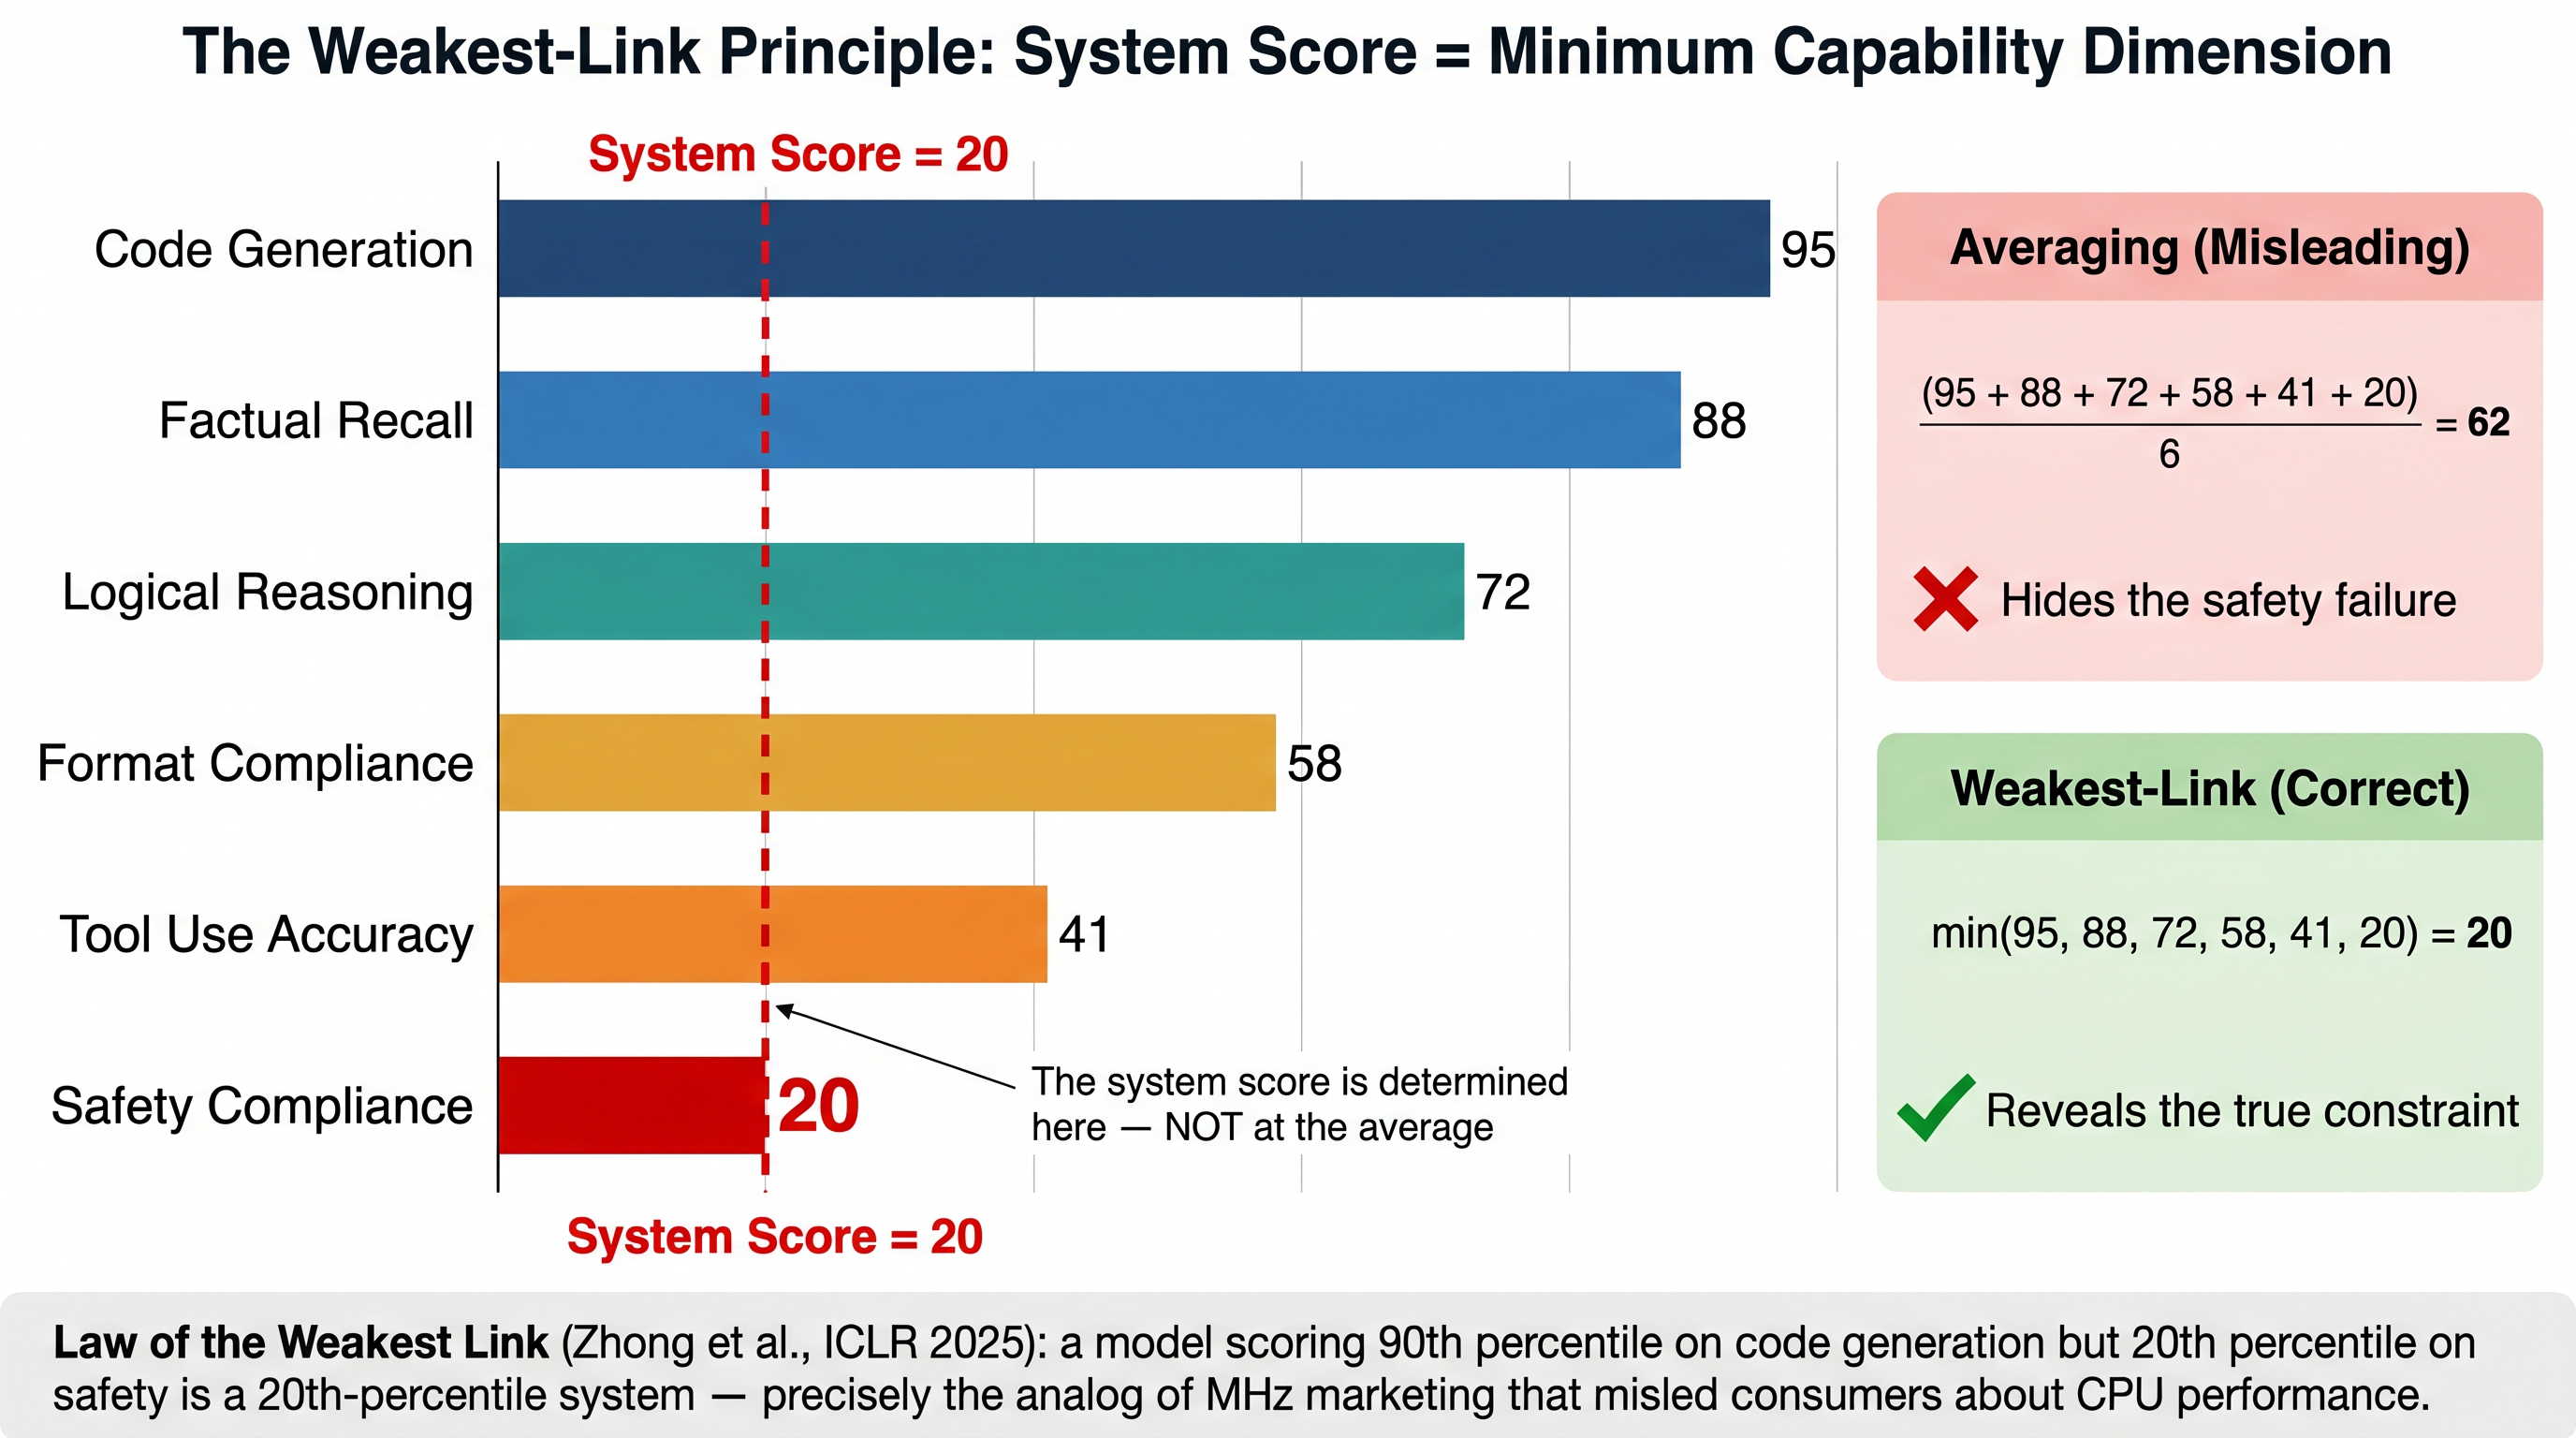
\includegraphics[width=0.80\textwidth]{figures/generated/fig_paradigm_bucket}
  \caption{The Bucket Principle (Law of the Weakest Link) applied to intelligent system evaluation.
  A system's capability is constrained by its weakest dimension, not its average.
  A model scoring 95th percentile on code generation but 20th percentile on safety
  has a system intelligence of the 20th percentile---the water level is set by the shortest stave.
  Average-case metrics (e.g., MMLU score) are as misleading as MHz marketing was for CPUs;
  worst-case, per-dimension evaluation is the correct analog of SPEC benchmarks.}
  \label{fig:paradigm:bucket}
\end{figure}


\subsection{The Intelligent Operating System: From Code to World}

\subsubsection{The Historical Arc: From Task-Specific Systems to General Operating Systems}

Early operating systems were not general-purpose. They were instruments built for particular missions: the FORTRAN Monitor System on the IBM 704 served scientific computing; Colossus-era systems served military encryption; early batch systems served payroll processing. No one would have described these systems as ``general'' operating environments. They were narrow, domain-specific tools that happened to manage hardware resources. This characterization maps precisely onto today's intelligent agent systems. Codex, Claude Code, and Devin are powerful, but they are narrowly scoped to software engineering workflows. They edit codebases, run terminals, manage file systems, and invoke APIs. They are, in historical terms, the FORTRAN Monitor Systems of intelligent computing: task-specific instruments that will later be recognized as precursors to something far more general.

The classical OS did not become general overnight. A sequence of capability inflections was required: multiprogramming (Atlas, 1962) enabled concurrent task execution; time-sharing (CTSS, 1961; Multics, 1965) made interactive computing possible; virtual memory and protected mode (Unix, VMS, 1970s) provided isolation and reliability; networking stacks (BSD TCP/IP, 1980s) connected systems; and hardware abstraction layers (Windows NT HAL, 1990s) decoupled the OS from specific hardware \cite{ritchie_thompson_1974, corbato_1962_ctss, corbato_1965_multics}. Each layer was necessary before a single OS could serve scientific computing, office automation, real-time control, and multimedia simultaneously.

Current intelligent systems occupy what might be called the programming-language stage of their evolution. Just as early OS ran assembly or single-language programs for specific hardware, today's agent OS runs ``prompt programs'' for specific domains, predominantly code. The leap to a general intelligent OS, one that orchestrates agents across robotics, autonomous driving, engineering, agriculture, entertainment, and space navigation, requires the same kind of abstraction-layer breakthroughs that separated Unix from its single-language, single-hardware predecessors.

The five-generation framework documented earlier traces the arc from batch processing (Gen~I) through governed OS (Gen~V). But the trajectory points beyond Gen~V toward what might be called Generation~VI: the general intelligent OS that interfaces with the full physical and digital world. Patterson and Hennnessy argue that the ISA was the foundational abstraction enabling hardware/software co-evolution \cite{patterson_hennessy_2017}. Hennessy and Patterson's 2019 Turing Lecture identifies open ISAs and domain-specific co-design as pillars of a ``new golden age'' \cite{hennessy_patterson_2019}. The same structural requirement, namely an open, well-specified interface between layers, will govern the transition from today's code-only agent OS to tomorrow's world-spanning intelligent OS.

\subsubsection{Compute-Substrate Agnosticism: The ISA Decoupling Principle Generalized}

The preceding subsection chronicled recent advances in neuromorphic, biological, compute-in-memory, and quantum substrates. This subsection addresses a more fundamental architectural question: \textbf{why should the intelligent OS be agnostic to the physical implementation of its compute core?}

The answer follows directly from the lessons of ISA abstraction \cite{patterson_hennessy_2017}. The ISA is the most important abstraction in classical computing not because any single implementation is superior, but because it allows the software ecosystem and the hardware ecosystem to \textbf{evolve independently}. ICA's interface contracts generalize this principle to model-native computing: if a compute core, whether a silicon GPU, a neuromorphic chip, a compute-in-memory substrate, or a biological neural network, can meet a defined intelligence-score threshold (discussed in the next subsection), it should be capable of running the intelligent OS. The OS and compute core are fully decoupled, just as Linux and the CPU are decoupled via the ISA.

The philosophical extension follows the RISC-V open-ISA philosophy \cite{hennessy_patterson_2019}: any hardware meeting the specification can run the software, regardless of its physical implementation. Even a trained biological network (a rat brain organoid that passes the intelligence-score threshold) could in principle serve as a compute core for the intelligent OS. The same orchestration layer that schedules Claude Code sub-agents on an NVIDIA H100 today could schedule sensorimotor tasks on a Cortical Labs CL1 tomorrow \cite{cortical_2025_cl1}, provided both cores satisfy the same interface contract. This is \textbf{substrate agnosticism} in its fullest form: the OS does not care whether its compute cores are etched in silicon or grown in a petri dish.

\subsubsection{Intelligence Scoring as ISA Compliance}

The preceding subsection established the bucket principle and worst-case evaluation as theoretical foundations. This subsection shifts perspective from ``how to evaluate a core'' to ``how to enforce the ISA contract through scoring.''

ISA compliance testing is the mechanism by which the hardware--software contract is enforced. A chip cannot claim to implement x86 unless it passes a comprehensive validation suite covering every instruction, every privilege mode, every edge case. Without this testing, the ISA contract is meaningless. By direct analogy, an intelligence scoring standard is the enforcement mechanism for the Intelligent ISA. Without it, substrate agnosticism collapses into untestable claims.

The ``Law of the Weakest Link,'' formalized by Zhong et al.\ at ICLR 2025, provides theoretical grounding for the strictness this enforcement demands \cite{zhong_2024_weakest_link}: when multiple capabilities must combine to produce reliable behavior, overall system performance is constrained by the weakest individual capability. A system that scores 95th percentile on code generation but 20th percentile on safety compliance has a system intelligence of the 20th percentile. The lowest stave in the bucket determines the water level.

This means that \textbf{without a bucket-principle scoring standard, substrate agnosticism is dangerous}. A biological compute core that passes 9 of 10 safety dimensions but fails on the tenth could be deployed as ``compliant'' under averaging-based metrics, creating catastrophic risk. Minimum-score enforcement is not merely a testing preference; it is a safety imperative. Just as empirical work has demonstrated that microarchitecture matters more than ISA alone, intelligence scoring must evaluate implementation quality, not merely interface compliance.

\subsubsection{OS-Level Heterogeneous Scheduling: From Energy Models to Capability-Cost Models}

The preceding subsections established the microarchitectural analogy for heterogeneous model orchestration. This subsection shifts one layer up: when heterogeneous cores are unified under an intelligent OS, how should \textbf{the scheduling policy itself} be designed?

Classical operating systems provide the complete architectural blueprint. Energy Aware Scheduling (EAS), merged into Linux kernel 5.0 in 2019, equips the OS scheduler with an Energy Model that predicts the cost of placing each task on each available CPU \cite{eas_linux_2019}. The intelligent OS analog is a \textbf{Capability-Cost Model} that predicts the quality, latency, and dollar cost of routing each subtask to each available compute core, whether a large model, a small model, a neuromorphic chip, or a biological substrate, thereby enabling intelligence-optimal scheduling.

Two OS-level scheduling patterns merit particular attention:

\paragraph{Overutilization fallback.}
When the system is overloaded, EAS falls back to conventional SMP load balancing, sacrificing energy efficiency for throughput. The intelligent OS analog is a ``quality-at-all-costs'' fallback: when the agent system faces peak load, it routes tasks to larger, more expensive models regardless of cost optimization.

\paragraph{Real-time telemetry and dynamic routing.}
Intel's Thread Director (Alder Lake, 2021) provides the OS scheduler with real-time hardware telemetry about thread behavior. The intelligent OS analog is a \textbf{Task Director} that monitors subtask characteristics in real time, including reasoning depth, safety sensitivity, and latency tolerance, and dynamically re-routes to the optimal compute substrate mid-execution.

The introduction of biological and neuromorphic substrates makes the scheduling challenge qualitatively harder. A biological core may have fundamentally different latency profiles, failure modes, and capability signatures than a silicon GPU. The intelligent OS scheduler must accommodate not merely ``fast versus slow'' but ``probabilistic versus deterministic,'' ``high-bandwidth versus low-latency,'' and ``silicon versus biological.'' This is heterogeneous scheduling at a level of complexity that classical OS designers never confronted, yet the architectural patterns (Energy Models, overutilization fallbacks, and real-time telemetry) are directly inherited from the big.LITTLE playbook.
Figure~\ref{fig:paradigm:scheduling} places the two scheduling architectures side by side.
\begin{figure}[htbp]
  \centering
  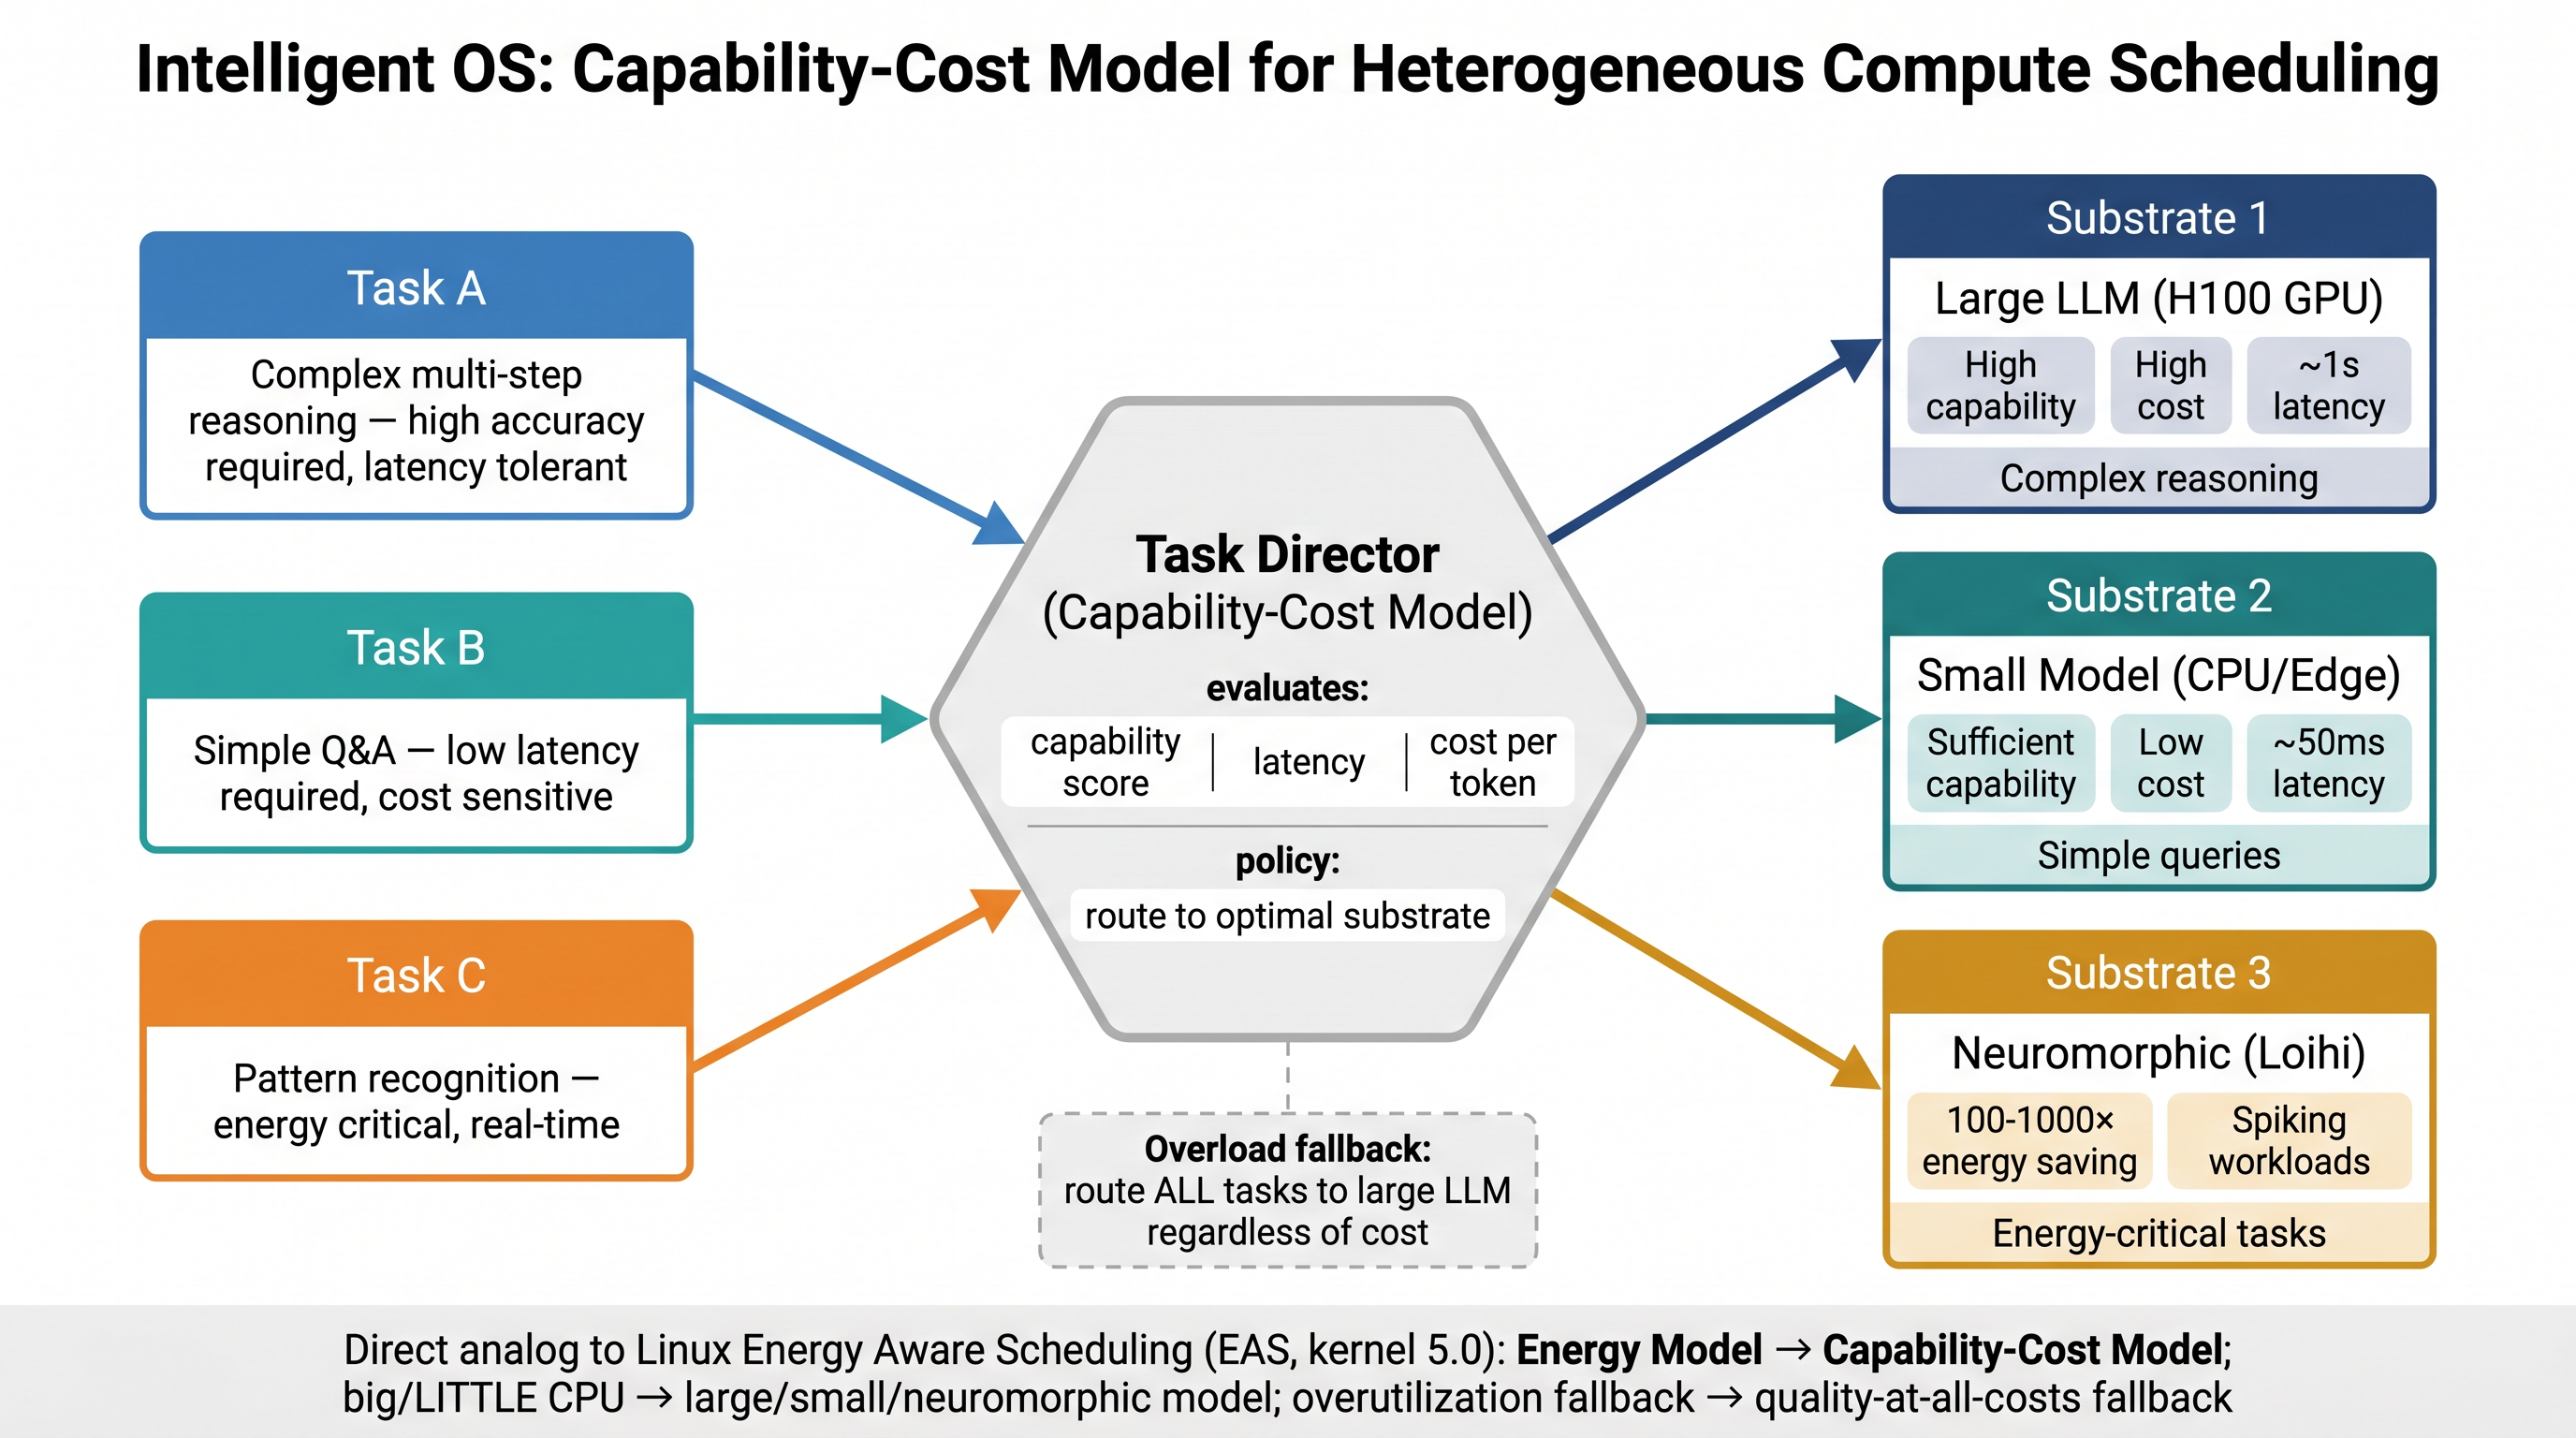
\includegraphics[width=0.88\textwidth]{figures/generated/fig_paradigm_scheduling}
  \caption{OS-level heterogeneous scheduling: Linux Energy Aware Scheduling (EAS) versus the intelligent OS Capability-Cost Model.
  EAS (Linux 5.0, 2019) uses an Energy Model to route each task to the most energy-efficient capable CPU
  and falls back to load balancing under overutilization.
  The Capability-Cost Model is the direct analog: a Task Director routes each subtask to
  the optimal compute core (large model, small model, neuromorphic, or biological substrate)
  by predicted capability, latency, and cost, falling back to the highest-capability core under peak load.}
  \label{fig:paradigm:scheduling}
\end{figure}


\subsubsection{The Physical World Interface: From Code-Only to Embodied Intelligence}

Today's intelligent OS interfaces with one domain: software engineering. Codex, Claude Code, and Devin operate on codebases, terminals, file systems, and APIs. In the historical framing established above, this is the FORTRAN Monitor System stage of intelligence: a task-specific OS for a single world. The next inflection is an intelligent OS that interfaces with the physical world: robotics, autonomous driving, engineering simulation, agriculture, entertainment, and space navigation.

Whole-brain emulation milestones are making embodied intelligence concrete. The FlyWire consortium mapped Drosophila's approximately 140,000 neurons and millions of synapses \cite{flywire_2024}, providing a complete connectome that enables detailed simulation of insect-scale neural circuits. These milestones demonstrate the trajectory toward more complex embodied agents that simulate complete organisms interacting with virtual environments.

A compute-substrate-agnostic intelligent OS means that the same orchestration layer that schedules Claude Code sub-agents today could, in principle, schedule robotic manipulation tasks, agricultural monitoring agents, and autonomous driving planners tomorrow. The requirements are twofold: the compute cores must meet the intelligence-score threshold (the bucket principle discussed above), and the OS must have appropriate world-interface drivers, such as sensors, actuators, simulation environments, and telemetry feeds.

This is the direct analog of how classical operating systems expanded from batch processing to real-time control. Unix started as a text-processing system, but the addition of real-time scheduling, device drivers, and networking stacks enabled it to run factory automation, telecommunications switches, and spacecraft guidance. Each new world required new driver interfaces but not a new OS kernel. The same Linux kernel runs a web server, a factory robot, and a Mars rover.

ICA's L4 (Semantic Interface Layer) and L5 (Orchestration Layer) are designed for this extensibility. Tool schemas and agent protocols are the device drivers of the intelligent OS. Adding a robotic arm driver or a satellite telemetry interface follows the same abstraction pattern as adding an MCP tool server today. The interface contract is consistent: sense, plan, act, verify, whether the target is a codebase or a cornfield.

Biological computing substrates add a unique dimension to embodied intelligence. Biological neural networks may possess natural advantages for sensorimotor tasks, pattern recognition, adaptive control, and real-time responsiveness that silicon-based systems lack. Kagan et al.\ (2022) demonstrated that biological neurons can learn to play Pong via feedback \cite{kagan_2022_pong_bioneurons}, confirming the viability of embodied bio-computing. The intelligent OS should be capable of dispatching sensorimotor subtasks to biological cores while routing symbolic reasoning to silicon GPUs, applying heterogeneous scheduling to embodied cognition. The scheduler picks the right core for the right task, just as a classical OS dispatches floating-point operations to the FPU and integer operations to the ALU. The physical world is not a different operating system; it is a different set of drivers for the same one.
